\section{Isolated Prompt Photons and Purity}
 
\subsection{Photon Sources}
Prompt photons can be defined simply as the photons produced promptly in the collision, before final state hadrons are produced. At the lowest order in pQCD, prompt photons are produced via two processes: (i) quark-gluon Compton scattering, $qg \to q\gamma$, (ii) quark-antiquark annihilation, $q\overline{q} \to g\gamma$, and, with a much smaller contribution,  $q\overline{q}\to$ $\gamma\gamma$. In addition, prompt photons are produced by higher-order processes, such as fragmentation or bremsstrahlung \cite{AURENCHE199334}. The collinear part of such processes has been shown to contribute effectively also at lowest order.

%ALICE-Prompt: Photons not from hadronic decays
%PHENIX-Prompt: RIGHT FROM THE COLLISION (excludes fragmentation)
%Direct is the same in both cases.
%%%%%LEADING ORDER FEYNMAN DIAGRAMS FROM QUAL%%%%%%%%%

Photons produced during fragmentation, the process by which a parton transforms into a spray of collimated final state particles called a jet, are aptly named fragmentation photons. As a result, fragmentation photons are often produced surrounded by a larger amount of energy and hadronic activity than other prompt photons produced from the initial hard scattering.

Prompt photons, and by extension fragmentation photons, are both included in the definition of direct photons. While the definition of direct photons is not always consistent in the literature, we define direct here to mean any photon not produced from hadronic decays. Those photons originating from the decay of a hadronic bound state are defined as decay photons. The two largest sources of decay photons are the two-photon decay channels of the $\pizero$ and $\eta$ meson.\\

Together, direct and decay photons make up all the photons observed in a collision, called inclusive photons.

$$ \gamma_\mathrm{inclusive} = \gamma_\mathrm{direct} + \gamma_\mathrm{decay}$$


A key challenge of this measurement is the relatively small cross section of prompt photons compared to decay photons. In order to reduce the background of decay photons, and to identify prompt photons, a combination of isolaton and electromagnetic shower profile selections are made.

%Also included in the definition of direct photons are thermal photons. These photons are produced as thermal radiation emitted by the quark gluon plasma. Thermal photons dominate the direct photon spectrum at low \pt, and at energies much lower than the photons of interest in this measurement (Section \ref{sec:photon_selection}).

\subsection{Photon Isolation Requirement}
\label{sec:isolation}
At leading order in pQCD, prompt photons are produced in 2$\to$2 processes surrounded by very little hadronic activity, in contrast to fragmentation photons found within a jet. Beyond leading order, the direct and fragmentation components cannot be factorized. As a result, the sum of their cross sections becomes the physical observable.\\

Despite this, the contribution from fragmentation photons can be suppressed by enforcing an isolation criteria, where the energy surrounding a photon must be less than a certain threshold. 
Theoretical calculations can also be simplified through the use of an isolation requirement. \cite{PhysRevD.82.014015}. This also has the benefit of suppressing the background from decays of neutral mesons often found within jets.

The simplest definition of isolation is defined as the scalar sum of the transverse momentum of charged particles within an angular radius, $R =\sqrt{(\Delta\varphi)^{2} +(\Delta\eta)^{2}  }$, around the cluster direction. This measurement uses $R = 0.4$, which is a common value used in various jet measurements.

\begin{equation}
\pt^\mathrm{iso,raw} = \sum_{\mathrm{track}~\in\Delta R<0.4} p_{\mathrm{T}}^{\mathrm{track}}	
\end{equation}

This does not, however, take into account the energy arising from the underlying event, described in the following section.
%Define underlying event


\subsection{Underlying Event Estimation for Photon Isolation}
\label{sec:ue_isolation}
The underlying event is defined as the sum of all processes that make up the final hadronic state in a collision, excluding the leading order hard scattering. This can include beam fragments, multi-parton interactions, and both initial and final state radiation. Essentially, the underlying event is made up of all the particles not directly associated with the hard scattering of the collision.

Here we describe the method used to estimate the underlying event for the purposes of correcting the isolation requirement. Later in Section \ref{sec:ue_subtraction}, the contribution from the underlying event to the azimuthal correlation measurement is described.

We use the jet area/median method which estimates the underlying event energy density,~$\rho$, from the median of the distribution of the transverse momentum densities of the jets in the event ~\cite{Cacciari:2009dp}. Jets are reconstructed by running the $k_\mathrm{T}$ reconstruction algorithm over all charged particles in the event, using a resolution parameter of R = 0.3. The transverse momentum density of each jet is simply the momentum of the jet divided by its area, determined by the sum of the voronoi cells of each particle within the jet\footnote{The voronoi cell is the region for each "seed", or particle, that  consists of all points in the same  plane that are closer to that seed than to any other.}. 
 This median calculation is described in Equation \ref{eq:ue_density}:

\begin{equation}
\label{eq:ue_density}
  \rho = \mathrm{med} \left\{ \frac{\sum_{i\in J'_k}
    p_{T,i}}{\sum_{i\in J'_k} A_i} \right\}
\end{equation}
where $p_{T,i}$ is the transverse momentum, and $A_i$ the Voronoi area of the particle $i$ within the jet reconstructed for UE estimation purpose $J'_k$. The median is determined from all jets in the event with the important exception of the two leading (highest moment) jets in the event, as those are most often associated with the hard scattering of the collision. This therefore assumes that most of the charged particles in the event is made up of soft particles, and that the charged particles originating from the hard scattering of the collisions are reasonably contained within the leading jets of the event ~\cite{Cacciari:2009dp}.

The charged-particle density, $\rho$, is calculated for each event; average values are 3.2 \GeVc~in photon- triggered events in \pPb~and 1.6 \GeVc~in pp collisions.

%TODO: Pull up a pp and p-Pb NTuple and just pull out the ue estimate branches for a quick plot here.


%TODO: Write about lack of neutrals in isolation
%isolation variable does not include neutral particles. This enables us to use the full acceptance of the EMCal and reduces biases arising from correlation with the opening angle of $\pi^{0}$ decays. However, it does result in a slightly lower purity of the isolated single photon signal. 

\subsection{UE Correction to Isolation Variable}
\label{sec:ue_correction_isolation}
For each event and cluster, we subtract the underlying event using the measured charged-particle density $\rho$ that is calculated event-by-event as described in Section~\ref{sec:ue_isolation}:

%For the determination of the isolation criterium,~$\pt^\mathrm{iso}$, the background due to the underlying event is estimated with the Voronoi method from the \textsc{FastJet} jet area/median package~\cite{Cacciari:2009dp} on an event-by-event basis and subtracted according to:

The result is an average subtraction for the isolation cone of {$R=0.4$} is about {$1.6$ \GeVc} and {$0.8$ \GeVc} for \pPb~and pp collisions, with a standard deviation of {0.9 \GeVc} and {0.4 \GeVc}, respectively.  

%A requirement of $\pt^\mathrm{iso}<1.5$ \GeVc is used, which results in a signal efficiency of about 90$\%$ that does not significantly depend on the photon $\pt$. 
 
For photons near the edge of the detector, the isolation energy requirement is scaled to account for any missing area in the isolation cone\footnote{The final isolated photon-hadron correlations are normalized to the number of reconstructed photons. As a result, the $\gammaiso$ efficiency was not studied in detail}. A check on on this scaling procedure was also done, and is shown in Section \ref{sec:iso_acceptance_check}. 

\begin{equation}
p_T^\mathrm{iso} = p_T^\mathrm{iso,raw} - \rho\times\pi(0.4)^{2}.
\end{equation}

Figure~\ref{fig:iso_ue} shows the isolation distribution before and after underlying event subtraction for \pPb~and pp collisions. The distributions have a positive tail that decreases exponentially; this is expected as this observable effectively measures multi-jet production. The difference between the \pPb~and pp distribution at low $\iso$ values can be attributed to the effect of enhanced soft-particle production in \pPb~collisions. The underlying event subtraction modifies the isolation distribution only slightly. After subtraction, the distributions show a negative tail, which arises from a over-subtraction of the underlying event due to region-to-region fluctuations. In both cases, this tail falls by more than three orders of magnitude by $\iso=-3$ \GeVc, indicating that over-subtraction is a small effect.   

\begin{figure}[h]
\center
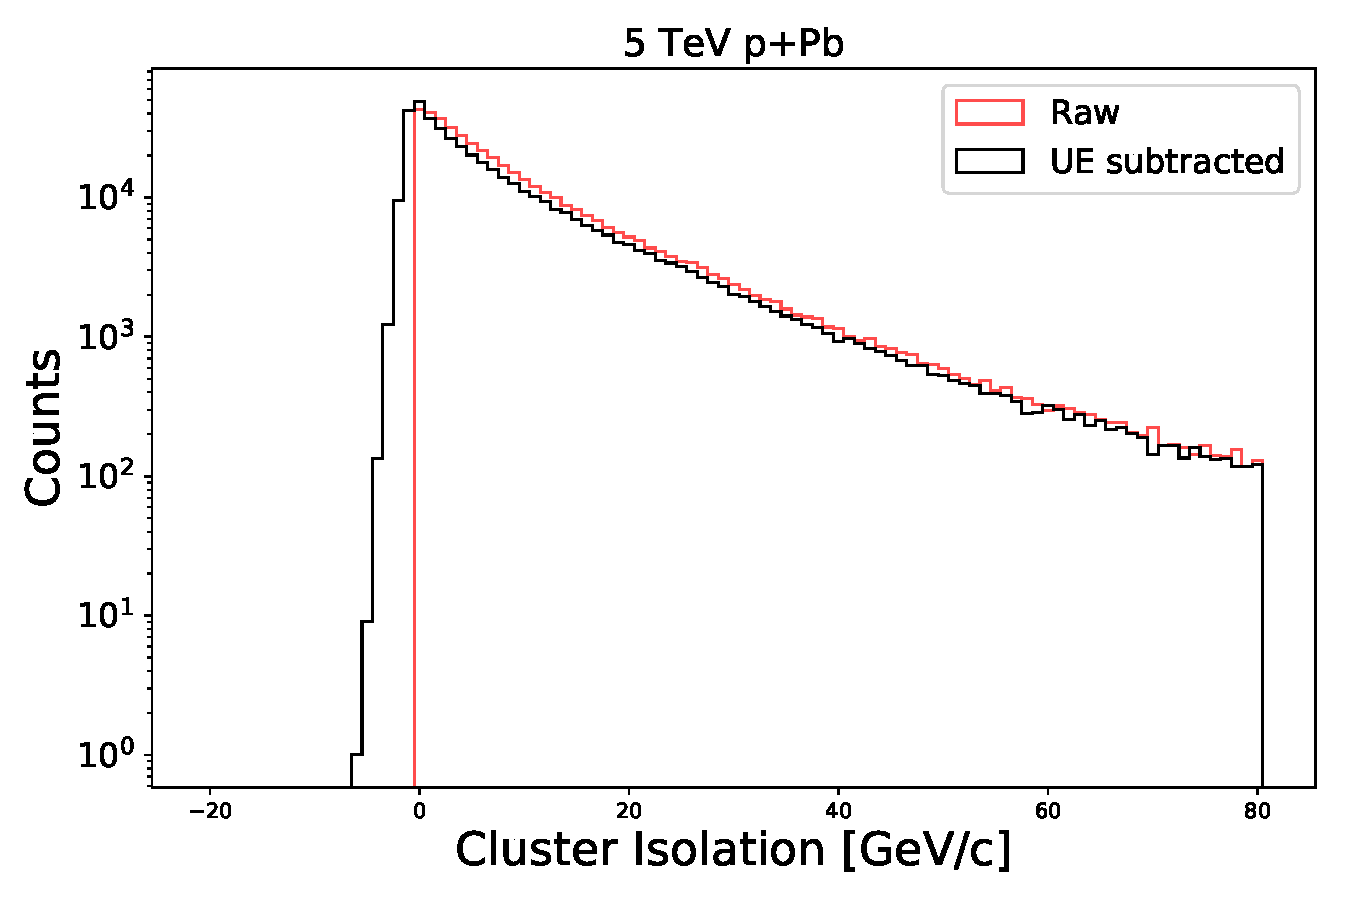
\includegraphics[width=0.49\textwidth]{Data_Analysis/Isolation/IsolationWithUESubtraction_Skimmed_13def_root}
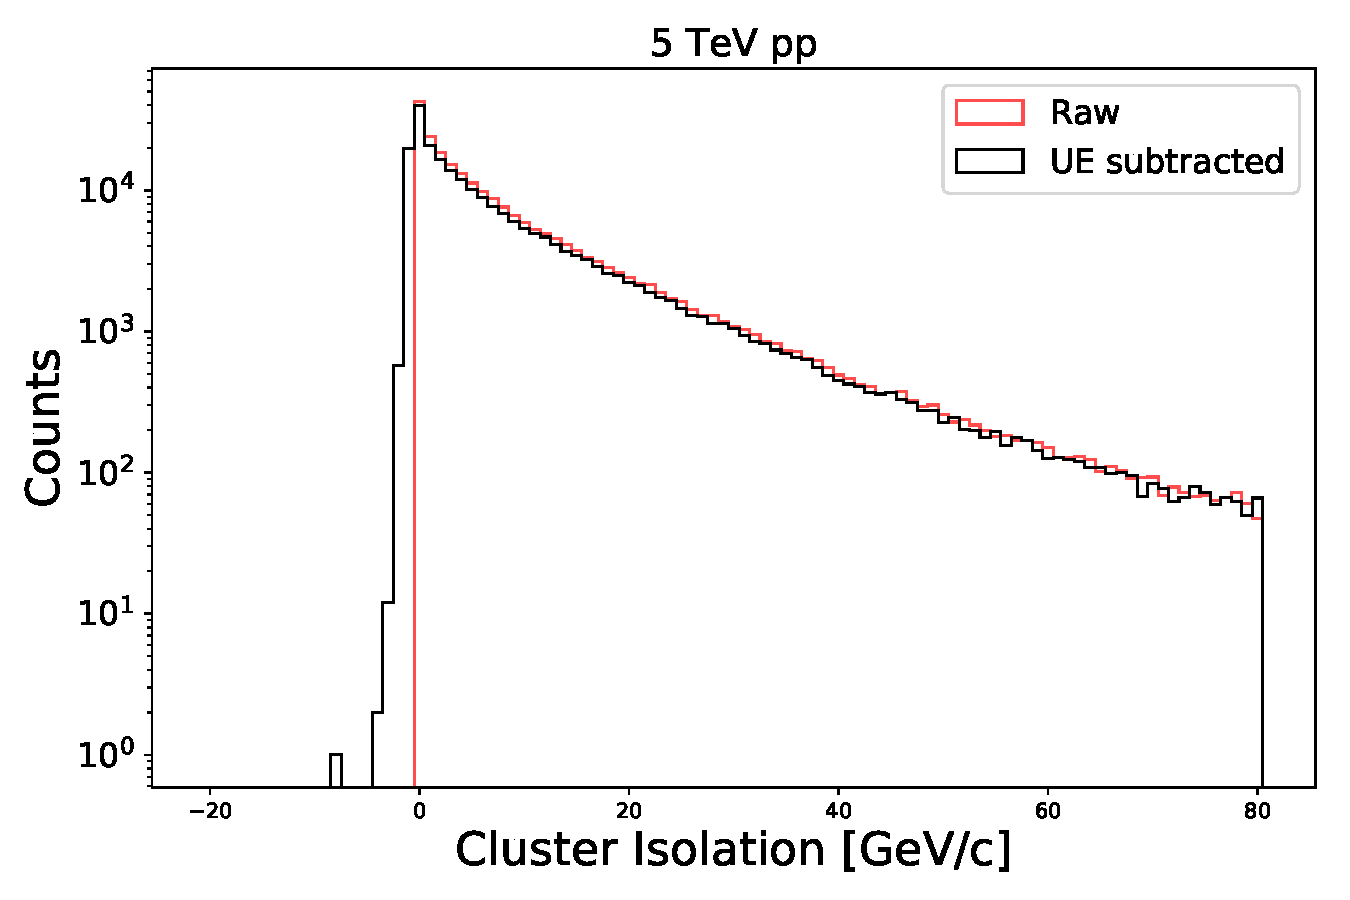
\includegraphics[width=0.49\textwidth]{Data_Analysis/Isolation/IsolationWithUESubtraction_Skimmed_17q_root}
\caption{Cluster isolation before and after underlying event subtraction in \pPb~(left panel) and pp (right panel) collisions.}
\label{fig:iso_ue}
\end{figure}

%TODO Fix Table Reference
Figure~\ref{MC_Isolation} shows the distribution of cluster isolation after UE subtraction for photon-jet and dijet simulations of \pPb~data (see Table~\ref{tab:MCsamples}). As expected, the distributions are rather different: whereas the dijet simulation shows a prominent exponential tail at large $\iso$ values, the photon-jet simulation shows a Gaussian-like shape that is mostly symmetrical except for a very small fraction of events that have large $\iso$ values. In both cases, the negative tail falls rather sharply, which is expected as it arises from region-to-region fluctuations of the UE that are independent of the hard-process involved. 

\begin{figure}[h]
\center
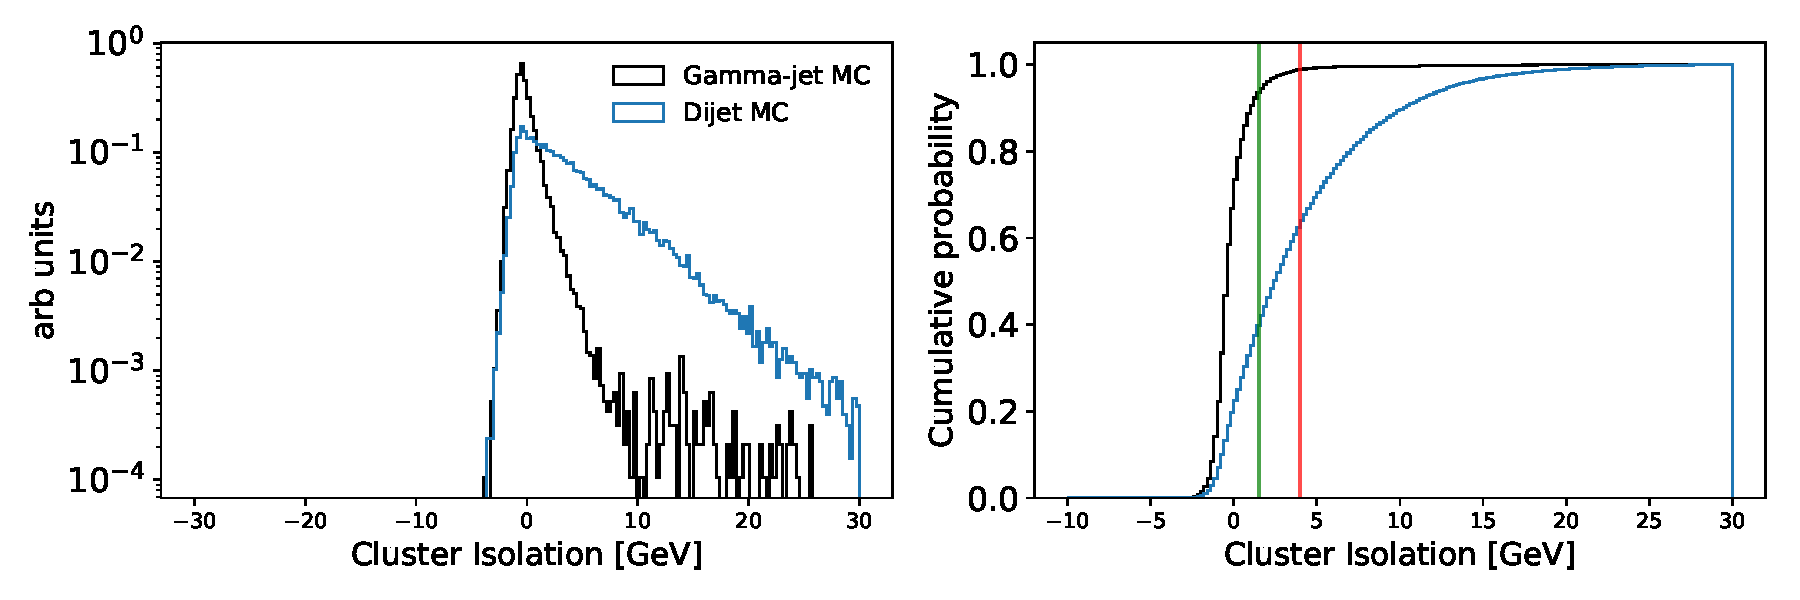
\includegraphics[width=1.0\textwidth]{Data_Analysis/Isolation/IsolationMCsignal_Skimmed_17g6a1_pthat1_4L_root}
\caption{Isolation distribution of clusters that pass our selection in \pPb~photon-jet and dijet simulations, and corresponding cumulative distribution. Two vertical lines at $\iso=$ 1.5 \GeVc~(green) and $\iso=$ 5.0 \GeVc~are shown in the right panel for reference.}
\label{MC_Isolation}
\end{figure}

%For the purposes of template fitting, we also need to define a sideband that is dominated by background. For this we note that only about 1$\%$ of prompt photons of the photon-jet simulation have {$\iso>$ 5 \GeVc}. Given that the cross-section for prompt photons is about two orders of magnitude smaller than the background, this region is overwhelmingly dominated by background.   

The cumulative distributions (Figure~\ref{MC_Isolation}, right panel) show that a {$\iso<$ 1.5 \GeVc} selection keeps about 90$\%$ of the signal and rejects about 60$\%$ of the background. We use this relatively loose photon isolation criteria to reduce the dependence of the results on the details of the simulation of the detector noise, tracking resolution, and the underlying event. 


%TODO: Put shower shape section first?
This isolation cut of {$\iso<$ 1.5 \GeVc} is used in conjunction with the shower-shape cut to complete our isolated-photon selection or ``$\gammaiso$ selection''. We call ``$\gammaiso$-candidates'' the clusters that pass our isolated photon selection because it still leaves a significant fraction of background (about 40$\%$ of the cross section, as just shown). 

The main background present in our $\gammaiso$ selection is from multi-jet events where one jet typically contains a $\pi^{0}$ or $\eta$, which carries most of the jet energy, and is misidentified  as a photon because it decays into a photon pair that is collinear with respect to the EMCal cell granularity. Other sources of background arise from charged-to-neutral fluctuations of jet fragmentation that leads to low observable $\iso$ (that considers only charged-particles). 

This creates the need to measure the purity of our $\gammaiso$-candidate selection, which is described in Section~\ref{sec:purity}. 


\subsection{Shower Profile Selection}

The primary background for this measurement are photons from the 2-body decay channel of $\pizero$'s.

A \pizero with a higher \pt will decay  with a smaller opening angle between the two decay photons. As the opening angle becomes smaller, the electromagnetic showers from the decay photons get closer together in the EMCal until they begin to overlap. For this reason, photons from $\pi^0$ decays begin to merge into a single cluster in the EMCal above approximately 6~\GeVc. This cluster, made up of two showers from decay photons, will therefore tend to have a more elongated shower profile than a cluster resulting from a single, ideally prompt, photon. Thus, in order reject clusters produced by two photons from a meson decay, and select clusters from single photons, we select clusters using variables that encode the shape of the calorimeter shower. 

Since $\lambdasquare$ represents the profile of the shower of the cluster, it discriminates between clusters belonging to single photons, for which the $\lambdasquare$ distribution is narrow and symmetric, and merged photons from neutral-meson decays, for which the distribution is dominated by a long tail towards higher values. 

%A \pizero with sufficiently high \pt, approximately 6~\GeVc, a \pizero will decay into two photons with such a small opening angle, that their electromagnetic showers from the two photons in the ALICE EMCal significantly overlap. %significantly overlapping elecromagnetic showers in the calorimeter
%For this reason, the two showers from the two photons will appear in the ALICE EMCal as a single cluster.

%Thus, in order to select against this measurement's largest source of background, we require that clusters have a more symmetric shape in the EMCal.

A variable that encodes the shape of a clusters electromagnetic shower profile is \lambdasquare. The $\lambdasquare$ variable is the weighted root-mean-square of the shower energy along the major ellipse axis, and thus clusters with a symmetric shower profile will trend towards smaller values of $\lambdasquare$. $\lambdasquare$ is defined according to~Ref.~\cite{Abelev:2014ffa} as:
\begin{equation}
\lambdasquare = \frac{s_{\eta\eta}+ s_{\phi\varphi}}{2} + \sqrt{   \frac{(s_{\eta\eta} - s_{\phi\varphi})^{2}}{4} + s^{2}_{\eta\varphi}         },
\end{equation}
where $s_{ij} = \langle ij \rangle - \langle i \rangle\langle j \rangle$ are the covariance matrix elements; the $i,j$ are cell indices in $\eta$ and  $\varphi$ axes; $\langle ij \rangle$ and $\langle i\rangle$, $\langle j\rangle$ are the second and the first moments of the cluster position cell weighted as follows:
\begin{equation}
\mathrm{weight} = \mathrm{max}\left(\log(E_{\mathrm{cell}}/E_{\mathrm{cluster}}), w_{0}\right). 
\end{equation}

Following previous studies~\cite{Acharya:2018dqe}, we chose the cutoff in the log-weighting as $w_{0}=-4.5$, which means that cells that contain less than {$e^{-4.5} =$ 1.1$\%$} of the total cluster energy are not considered in the $\lambdasquare$ calculation.

Thus it discriminates between clusters belonging to single photons, for which the $\lambdasquare$ distribution is narrow and symmetric, and merged photons from neutral-meson decays, for which the distribution is dominated by a long tail towards higher values.

%TODO Include Isolation cartoon from Qual